\chapter{Classificazione e Designazione degli acciai}\label{chp:ClassAcc}
\section{La normazione}
Per cominciare, è utile osservare come gli enti di normazione descrivono gli acciai.
tra l'altro sono tra i prodotti più normati presenti sul mercato industriale.
Dapprima:
\begin{description}
\item[UNI] sigla che indica una normativa realizzata dall'Ente nazionale di Unificazione.
Ente che norma tutte le attività produttive sul mercato italiano. Inoltre è facente parte del \acs{CEN}. Difatti applica sul suolo italiano tutte le normative date dallo stesso \acs{CEN}.
Non è ammessa la presenza di normative che siano in contrasto con quelle europee.
\item[EN] contraddistingue le norma sviluppate dal \ac{CEN}.
Le normative EN devono essere percepite da tutti gli stati membri dello spazio economico europeo.
Ciò per garantire il libero scambio di prodotti al interno del mercato.
Il EN è composto dai principali enti nazionali di normazione degli stati membri nello spazio economico europeo.
\item[ISO] rappresenta tutte le normative sviluppate dal \ac{ISO}. Possono essere un riferimento applicabile per tutto il mondo. Una nazione può decidere se applicare le norma \acs{ISO} indipendentemente da quanto fatto dal \acs{CEN}.
\end{description} 

Secondo le normative della \acs{CEN} le normative hanno lo scopo di:
\begin{quote}
Stabilire le condizioni tecniche per lo scambio di prodotti e di servizi assicurando il continuo adeguamento allo sviluppo delle tecnologie e dei bisogni del mercato
\end{quote}
con lo scopo di eliminare le barriere commerciali, almeno tra gli stati europei.

Una prima classificazione dei tipi di acciai perché esistono tante classi di materiale.
Dunque si può pensare ad una divisione in base:
\begin{multicols}{2}
\begin{itemize}
\item composizione chimica;
\item processo di fabbricazione;
\item caratteristiche meccanico-fisiche e di impiego;
\columnbreak
\item costituenti strutturali;
\item ecc\dots
\end{itemize}
\end{multicols}

Non a caso sono stati citati i precedenti aspetti, in fatti le normative vanno a coprire gli aspetti stessi, come mostrato nella tabella \ref{tab:NormGen}

\begin{table}
\centering
\caption{Norme di carattere geneale}\label{tab:NormGen}
\begin{tabularx}{\textwidth}{>{\bfseries}lX}
\toprule
UNI EN 10020:2001 & Descrizione e classificazione dei tipi di acciaio\\
UNI EN 10027-1:2016 & Sistemi di designazione degli acciai, \texttt{Designazione alfanumerica}\\
UNI EN 10027-2:2015 & Sistemi di designazione degli acciai, \texttt{Designazione numerica}\\
UNI EN 10025-(1-6):2005 & Prodotti laminati a caldo di acciai per impieghi strutturali\\
UNI EN 10079:2007 & Descrizione dei prodotti di acciaio (forma, dimensioni, aspetto, stato superficiale)\\
\bottomrule
\end{tabularx}
\end{table}

Secondo la norma \texttt{UNI EN 10020:2001}:
\begin{quote}
L'acciaio è un materiale il cui \emph{tenore in massa di Ferro (Fe) è maggiore di quello di ciascuno degli altri elementi} ed il cui \emph{tenore di Carbonio (C) è generalmente minore del $2\%$} e che contiene altri elementi. Un numero limitato di acciai al Cromo (Cr) può avere tenore di carbonio maggiore del $2\%$, ma tale valore del $2\%$ è il tenore limite corrente che separa l'acciaio dalla ghisa.
\end{quote}
Sempre la stessa norma definisce la classificazione principale degli acciai \ref{fig:UNIEN10020:2001}.

\begin{figure}
\usetikzlibrary{trees}
\begin{tikzpicture}[
sibling distance = 10em,
every node/.style={rectangle, rounded corners, draw, align=center,}
]
\node{Acciai}
	child{ node[top color = UnifeLight] {Non legati}
		child{ node[bottom color = UnifeDark!80, white] {di qualità}}
		child{ node[bottom color = UnifeDark!80, white] {speciale}}}
	child{node[top color = UnifeLight] {Inossidabili}}
	child{node[top color = UnifeLight] {Legati}
		child{node[bottom color = UnifeDark!80, white] {di qialità}}
		child{node[bottom color = UnifeDark!80, white] {speciali}}};
\end{tikzpicture}
\caption{Suddivisione acciai in base alla normativa UNI EN 10020:2001}
\label{fig:UNIEN10020:2001}
\end{figure}
Dove:
\begin{itemize}
\item \textcolor{UnifeLight}{$\blacksquare$} è la suddivisione per composizione chimica;
\item \textcolor{UnifeDark!80}{$\blacksquare$} è la suddivisione in base alle caratteristiche meccanico-fisiche della suddivisione chimica.
\end{itemize}
L'appartenenza ad una classe si basa sulla composizione chimica di colata indicata sulla norma di prodotto, prendendo in considerazione il valore minimo.
Vediamo ora come vengono suddivise le categorie in base alla norma.
\begin{description}
\item[Acciai non legati] sono gli acciai per cui \emph{Nessuno dei valori limite, rigorosamente fissati dalla norma (tabella \ref{tab:Prosp1}), è raggiunto dai rispettivi tenori degli elementi in lega} (escluso il C).
\item[Acciai inossidabili] sono acciai contenenti \emph{almeno il $10.5\%$ di Cr e al massimo l'$1.2\%$ di C}.
\item[Acciai legati] sono acciai per i quali \emph{almeno uno dei valori limite è raggiunto dai dai rispettivi tenori degli elementi in lega} (tabella \ref{tab:Prosp1}) a patto che non siano già appartenenti agli inossidabili.
\end{description}

\begin{table}
\centering
\caption{Prospetto I, norma UNI EN 10020:2001}\label{tab:Prosp1}
\begin{tabularx}{0.5\textwidth}{lXl}
\toprule
\textbf{Elemento} &\textbf{Tenore in $\%$ in massa}\\
\midrule
Al & Alluminio & 0.30\\
B & Boro & 0.0008\\
Bi & Bismuto & 0.10\\
Co & Cobalto & 0.30\\
Cr & Cromo & 0.30\\
Cu & Rame & 0.40\\
La & Lantanidi (singolarmente) & 0.10\\
Mn & Manganese & 1.65\\
Mo & Molibdeno & 0.08\\
Nb & Niobio & 0.06\\
Ni & Nichel & 0.30\\
Pb & Piombo & 0.40\\
Se & Selenio & 0.10\\
Si & Silicio & 0.60\\
Te & Tellurio & 0.10\\
Ti & Titanio & 0.05\\
V & Vanadio & 0.10\\
W & Tungsteno & 0.30\\
Zr & Zircronio & 0.05\\
- & Altri & 0.10\\
\bottomrule
\end{tabularx}
\end{table}

\subsection{Acciai non legati}
\begin{multicols}{2}[]
\subsubsection{Di Qualità}
Sono acciai per i quali, in genere, sussistono prescrizioni riguardanti caratteristiche specifiche, per esempio: tenacità, grossezza e/o formabilità.
Non sono destinati a trattamenti termici (al più a ricottura e normalizzazione).
\columnbreak
\subsubsection{Speciali}
Sono acciai che presentano, rispetto agli acciai non legati di qualità, una maggiore purezza in particolare nei confronti delle inclusioni non metalliche.
In genere presentano risposta regolare ai \ac{TT}, e nella maggior parte dei casi sono destinati a:
\begin{enumerate}
\item trattamento di bonifica,
\item trattamento di tempra superficiale.
\end{enumerate}
Fanno parte di tale classe gli acciai non legati che rispondono a una o più delle seguenti prescrizioni tutte quelle definizioni che rientrano in \ref{sec:ANLS}.
\end{multicols}

\subsection{Acciai inossidabili}
Sono suddivise in base a due criteri:
\begin{enumerate}
\item tenore di Nichel:
\begin{itemize}
\item Ni $<2.5\%$
\item Ni $>2.5\%$
\end{itemize}
\item caratteristiche paricolari:
\begin{itemize}
\item resistenza alla corrosione;
\item resistenza all'ossidazione a caldo;
\item resistenza allo scorrimento.
\end{itemize}
\end{enumerate}
\newpage
\subsection{Acciai legati}
\begin{multicols}{2}[]
\subsubsection{di Qualità}
Sono acciai il cui utilizzo è simile agli acciai non legati di qualità, ma che contengono elementi in lega per rispondere ad alcune prescrizioni di impiego.
Non sono, di regola, destinati a trattamento termico di bonifica o ad un tratamento di tempra superficiale.
Ne fanno parte gli acciai definiti in \ref{sec:ALDQ}.
\columnbreak
\subsubsection{Speciali}
Sono acciai , diversi dagli inossidabili, che non rientrano tra le categorie definite per gli acciai legati di qualità caratterizzati da:
\begin{itemize}
\item regolazione precisa della composizione chimica;
\item particolari condizioni di elaborazione e controllo del processo produttivo.
\end{itemize}
Ne fanno parte gli acciai descritti in \ref{sec:ALS}.
\end{multicols}

\section{La norma UNI EN 10027-1:2016}\label{sc:10027-1}
La normativa ha lo scopo di designare univocamente gli acciai disponibili in commercio in base a due modalità: designazione alfanumerica (parte 1) e designazione numerica (parte 2).
Inoltre specifica le modalità di nomenclatura degli acciai: specificando le modalità di ottenimento dei nomi per entrambe le parti%
\footnote{Come nominare un acciaio non viene deciso dall'azienda che lo produce. Lo stesso ente ha il compito di nominare gli acciai.}.
Inizieremo dalla prima parte ovvero quella alfanumerica.

\subsection{UNI EN 10027-1 gruppo 1:2016}\label{ssc:10027-1Gruppo1}
Nella prima parte della normativa vengono designati gli acciai in base al loro impiego e alle loro caratteristiche meccanico-fisiche.
Alla figura \ref{tab:Simb} è rappresentata la modalità di nomenclatura alfanumerica.

\begin{table}
\centering
\caption{Indicazioni simboli}\label{tab:Simb}
\begin{tabularx}{\textwidth}{p{0.2\textwidth}XXp{0.1\textwidth}}
\toprule
\textbf{W} & \textbf{X} & \textbf{YYY} & \textbf{ZZ}\\
Simbolo iniziale & Simbolo Impiego & Caratteristiche meccanico-fisiche & Altre indicazioni\\
\midrule
\begin{description}
\item[G]: Acciaio per getti 
\item[PM]: metallurgia delle polveri
\end{description}
&
\begin{description}
\item[S] Impieghi strutturali,
\item[P] Impieghi sotto pressione,
\item[E] Costruzioni meccaniche,
\item[D] Formatura a freddo,
\item[B] Cemento armato,
\item[Y] Cemento armato precompresso,
\item[R] Acciaio per rotaie,
\item[M] Acciai magnetici,
\item[\dots]\dots
\end{description}
&
\begin{description}
\item[$R_{s,min}$] in $\left[ \unit{\MPa}\right]$
\item[$R_{m,min}$] in $\left[\unit{\MPa}\right]$
\item[$HBW_{min}$] (adimensionale)
\end{description}
&
Simboli addizionali divisi in due gruppi
\\
\bottomrule
\end{tabularx}
\end{table}

Come si vede dalla tabella \ref{tab:Simb} i vari simboli occupano una posizione ben determinata e specifica.
C'è da considerare una particolarità tra il simbolo d'impiego e il valore della caratteristica meccanico-fisica specificata per tale categoria.
\begin{description}
\item[In generale] viene specificato il valore di snervamento minimo garantito: $R_{s,min}\left[\unit{MPa}\right]$.
\item[Per Y] Viene specificata la tensione minima di rottura: $R_{m,min}\left[\unit{MPa}\right]$
\item[Per M] Viene indicata una proprietà magnetica (descritta dalla normativa).
\item[Per R] La durezza.
\end{description}
Per quanto riguarda le altre indicazioni, anche in questo caso dipende dal impiego del materiale.
Viene riportato un esempio in tabella \ref{tab:ValRes}.

\begin{table}
\centering
\caption{Valori di resilienza}\label{tab:ValRes}
\begin{tabularx}{\textwidth}{XXXX}
\toprule
\multicolumn{4}{c}{Resilienza}\\
\textbf{J} & \textbf{K} & \textbf{L} & \textbf{Temperatura}\\
min $27\unit{\J}$ & min $40\unit{\J}$ & min $60\unit{\J}$ & $\left[\unit{\celsius}\right]$\\
\midrule
JR & KR & LR & 20\\
J0 & K0 & L0 & 0\\
J2 & K2 & L2 & -20\\
\bottomrule
\end{tabularx}
\end{table}

\begin{example}{Descrizione acciaio}
Se consideriamo come esempio l'acciaio $S355J2$, questo sarà:
\begin{description}
\item[$S$] un acciaio per impieghi strutturali,
\item[$355$] avrà valore minimo di snervamento pari a $R_{s,min} = 355\unit{\MPa}$,
\item[$J2$] valore di resistenza minima a $27\unit{\J}$ ad una temperatura di $-20\unit{\celsius}$.
\end{description}\label{exa:DescrizoneAcciai}
\end{example}%
Si ricorda che la necessità si aggiungere un valore di riferimento alla resilienza, come mostrato all'esempio \ref{exa:DescrizoneAcciai}, è motivato dal fatto che: il valore di resilienza dipende dalla temperatura di esercizio del materiale in quanto la bassa temperatura tende a cristallizzare il metallo rendendolo più fragile.

Tra le altre cose il metallo appena visto è uno di quei metalli facente parte della normativa UNI EN 10025-2 ovvero per gli acciai \textit{prodotti laminati a caldo per impieghi strutturali}. Giusto per darne un accenno la normativa è divisa in sei parti:
\begin{enumerate}
\item Condizioni tecniche generali di fornitura
\item Condizioni tecniche di fornitura di acciai non legati per impieghi strutturali
\item Condizioni tecniche di fornitura di acciai per impieghi strutturali saldabili a grano fine allo stato normalizzato/normalizzato laminato
\item Condizioni tecniche di fornitura di acciai per impieghi strutturali saldabili a grano fine ottenuti mediante laminazione termomeccanica
\item Condizioni tecniche di fornitura di acciai per impieghi strutturali con resistenza migliorata alla corrosione atmosferica
\item Condizioni tecniche di fornitura per prodotti piano di acciai per impieghi strutturali ad alto limite di snervamento allo stato bonificato
\end{enumerate}

\subsection*{La normativa precedente: UNI EU 27/77}
Sebbene non più in vigore è utile visionare la vecchia normativa, in quanto molte aziende -anche al giorno d'oggi- utilizzano la vecchia nomenclatura.
Nello specifico, il gruppo 1, considerato anche nella normativa in vigore, si suddivideva in ulteriori due gruppi:
\begin{description}
\item[Sottogruppo 1.1] Designazione per caratteristiche meccaniche, di cui non si garantiva la composizione chimica.
\item[Sottogruppo 1.2] Designazione per tipo d'impiego. 
\end{description}
Inoltre, la normativa stessa poneva tali prodotti come venduti allo stato grezzo: stato di lavorazione a caldo, senza trattamento termico.

\subsubsection*{Sottogruppo 1.1}
\begin{table}
\centering
\caption{Sottogruppo 1.1 vecchia normativa}\label{tab:OldLaw1.1}
\begin{tabularx}{\textwidth}{|c|X|X|X|}
\toprule
\textbf{Fe} & \textbf{Simbolo iniziale} & \textbf{Caratteristica meccanica} & \textbf{Altre indicazioni}\\
\midrule
&
\begin{description}
\item[G] per acciaio per getti
\end{description}
&
\begin{description}
\item[$R_{m,min}$] Caratteristica a rottura in $\unit{\MPa}$
\item[$R_{s,min}$] Caratteristica a snervamento in $\unit{\MPa}$ solo preceduta da \textbf{E}
\end{description}
&\\
\bottomrule
\end{tabularx}
\end{table}

Alla tabella \ref{tab:OldLaw1.1} viene rappresentata la designazione degli acciai in base alla vecchia normativa. Le altre indicazioni, generalmente, contenevano il grado di insensibilità alla frattura fragile: indicata con le lettere dalla A alla D in ordine crescente di insensibilità; il simbolo dell'elemento chimico contenuto in bassi tenori; numeri da 1 a 3 che ne indicavano il grado qualitativo crescente.

\begin{example}{Sottogruppo 1.1}
\begin{multicols}{3}
\begin{itemize}
\item Fe360
\item FeE355
\columnbreak
\item Fe410Pb
\item Fe410D
\columnbreak
\item FeG450
\item Fe490-2
\end{itemize}
\end{multicols}
\end{example}

\subsubsection*{Sottogruppo 1.2}
\begin{table}
\centering
\caption{Sottogruppo 1.2 vecchia normativa}\label{tab:OldLaw1.2}
\begin{tabularx}{\textwidth}{|c|X|X|}
\toprule
\textbf{Fe} & \textbf{Lettera} & \textbf{Numero di due o più cifre}\\
\midrule
&
Indice d'impiego
&
È una specifica relativa al prodotto e ne indica il grado di qualità\\
\bottomrule
\end{tabularx}
\end{table}
Alla tabella \ref{tab:OldLaw1.2} è rappresentata la vecchia nomenclatura degli acciai secondo il loro impiego.

\begin{example}{Sottogruppo 1.2}
FeP03 era noto come acciaio in lamiera sottile per imbutiture (P) con grado di qualità 03
\end{example}

\subsection{UNI EN 10027-1 gruppo 2:2016}\label{ssc:10027-1Gruppo2}
Altre categorie di acciai, sempre classificandone il loro impiego sono:
\begin{enumerate}
\item Acciai non legati con tenore medio di Mn $<1\%$
\item Acciai non legati con tenore medio di Mn $>1\%$, acciai non legati per lavorazioni meccaniche ad alta velocità ("autmoatici"), acciai legati (no HS) con tenori di massa di ciascun elemento in lega $<5\%$
\item Acciai legati (No HS) il cui tenore in massa di almeno un elemento in lega sia $>5\%$
\item Acciai rapidi HS.
\end{enumerate}

\subsubsection{Sottocategoria 2.1}\label{sssc:Sottogruppo2.1}
Sono acciai non legati con tenore in massa di Mn $<1\%$

\begin{table}
\centering
\caption{Sottocategoria 2.1}
\label{tab:Sotto1}
\begin{tabularx}{\textwidth}{|c|X|X|}
\toprule
\textbf{C} & \textbf{$\%C \times 100$} & \textbf{Altre indicazioni}\\
\midrule
Se necessario \textbf{GC} se acciai per getti
&&
\begin{description}
\item[E] zolfo massimo stabilito
\item[R] zolfo in un dato intervallo
\item[U] Acciaio ottimizzato per utensili
\item[S] Acciaio ottimizzato per molle
\item[\dots] \dots
\end{description}\\
\bottomrule
\end{tabularx}
\end{table}

Alla tabella \ref{tab:Sotto1} è riportato la designazione degli acciai per questa sottocategoria.

\begin{example}{Sottocategoria 2.1}
C10 acciaio da carbo-cementazione\\
C40, C80, C120\\
C35E
\end{example}

\subsubsection{Sottocategoria 2.2}\label{sssc:Sottogruppo2.2}
Acciai non legati con tenore medio di Mn $>1\%$, acciai non legati per lavorazioni meccaniche ad alta velocità ("automatici"), acciai legati (no HS) con tenori in massa di ciascun elemento in lega $<5\%$. Alla tabella \ref{tab:Sotto2} viene riportata la formula

\begin{table}
\centering
\caption{Sottocategoria 2.2}\label{tab:Sotto2}
\begin{tabularx}{\textwidth}{|X|X|X|}
\toprule
\textbf{$\%C \times 100$} & \textbf{Simboli elementi in lega} & \textbf{Concentrazione degli elementi in lega}\\
\midrule
Se necessario \textbf{G} per gli acciai per getti &
In ordine decrescente di quantità &
Moltiplicati per il rispettivo fattore (vedi tabella \ref{tab:FattoriElementi})\\
\bottomrule
\end{tabularx}
\end{table}
I numeri relativi ai diversi elementi devono essere separati da trattini (non sempre vengono specificati tutti).

\begin{table}
\centering
\caption{Fattori moltiplicativi elementi}\label{tab:FattoriElementi}
\begin{tabularx}{\textwidth}{XX}
\toprule
\textbf{Elementi chimici} & \textbf{Fattore moltiplicativi}\\
\midrule
Cr, Co, Mn, Ni, Si, W & 4x\\
\midrule
Al, Be, Cu, Mo, Nb, Pb, Ta, Ti, V, Zr & 10x\\
\midrule
Ce, N, P, S & 100x\\
\midrule
B & 1000x\\
\bottomrule
\end{tabularx}
\end{table}

\begin{example}{Esempi di nomenclatura 2.2}
\begin{tabularx}{\textwidth}{XXX}
\multirow{4}{*}{35CrNiMo4-2-3} & $0.38\%$ & Carbonio\\
	& $1\%$ & Cr\\
	& $0.5\%$ & Ni\\
	& $0.3\%$ & Mo\\
\midrule
\multirow{2}{*}{34CrMo4} & $0.34\%$ & Carbonio\\
	& $1\%$ & Cr\\
\bottomrule
\end{tabularx}
\end{example}

\subsubsection{Sottocategoria 2.3}\label{sssc:Sottogruppo2.3}
Acciai legati (No HS) il cui tenore in massa di almeno un elemento in lega sia $>5\%$.
Nomenclatura è rappresentata in tabella \ref{tab:Sotto3}.

\begin{table}
\centering
\caption{Sottocategoria 2.3}\label{tab:Sotto3}
\begin{tabularx}{\textwidth}{|X|X|X|X|}
\textbf{X} & \textbf{$\%C \times 100$} & \textbf{Simboli elementi in lega} & \textbf{Concentrazione degli elementi in lega}\\
\midrule
Se necessario \textbf{GX} per acciai da getto o \textbf{PMX} per metallurgia delle polveri &&
In ordine decrescente di quantità &
Senza fattori moltiplicativi\\
\end{tabularx}
\end{table}

\begin{example}{Esempi di nomenclatura 2.3}
\begin{tabularx}{\textwidth}{XXX}
\multirow{3}{*}{X5CrNi18-8} & $0.05\%$ & Carbonio\\
	& $18\%$ & Cr\\
	& $8\%$ & Ni\\
\end{tabularx}
\end{example}

\subsubsection{Sottocategoria 2.4}\label{sssc:Sottogruppo2.4}
Acciai rapidi (HS).

\begin{table}
\centering
\caption{Sottocategoria 2.4}\label{tab:Sotto4}
\begin{tabularx}{\textwidth}{|X|X|}
\toprule
\textbf{HS} & \textbf{Concentrazione degli elementi in lega}\\
\midrule
Se necessario \textbf{PMHS} per metallurgia delle polveri &
Nell'ordine: W, Mo, V, Co\\
\bottomrule
\end{tabularx}
\end{table}
Gli acciai super-rapidi sono caratterizzati da 4 numeri \textbf{in quello specifico ordine}: \textbf{W, Mo, V, Co}.\\
Gli acciai rapidi e semi-rapidi sono caratterizzati da 3 numeri \textbf{sempre nello specifico ordine}: \textbf{W, Mo, V}.\\

\begin{example}{Esempi di nomenclatura 2.4}
\begin{tabularx}{\textwidth}{XXX}
\multirow{4}{*}{HS7-4-2-5} & $7\%$ & Tungsteno\\
	& $4\%$ & Molibdeno\\
	& $2\%$ & Vanadio\\
	& $5\%$ & Cobalto\\
\end{tabularx}
\end{example}

\section{La norma UNI EN 10027-2}\label{sc:10027-2s}
Vediamo da subito la nomenclatura per tali tipi di acciai alla tabella \ref{tab:ClassParte2}.
\begin{table}
\centering
\caption{Classificazione acciai su base chimica}
\label{tab:ClassParte2}
\begin{tabularx}{\textwidth}{|X|X|X|}
\toprule
\textbf{N.} & \textbf{XX} & \textbf{YY(ZZ)}\\
Numero di gruppo del materiale & Numero del gruppo dell'acciaio & Numero sequenziale in lega\\
\bottomrule
\end{tabularx}
\end{table}

Il numero del gruppo, nel caso degli acciai, è \textbf{1}. Altri numeri sono impiegati per altri tipi di metalli e leghe:

\begin{enumerate}
\item Acciai,
\item Metalli pesanti escluso l'acciaio (rame e leghe di rame)
\item Metalli leggeri (alluminio e leghe, Magnesio e leghe, ecc\dots)
\item \dots
\item Ghise
\item fino a 9 materiali.
\end{enumerate}

Alla figura \ref{fig:UNIEN10027-2} sono riportati i codici identificativi dei vari gruppi di acciai.

\begin{figure}
\centering
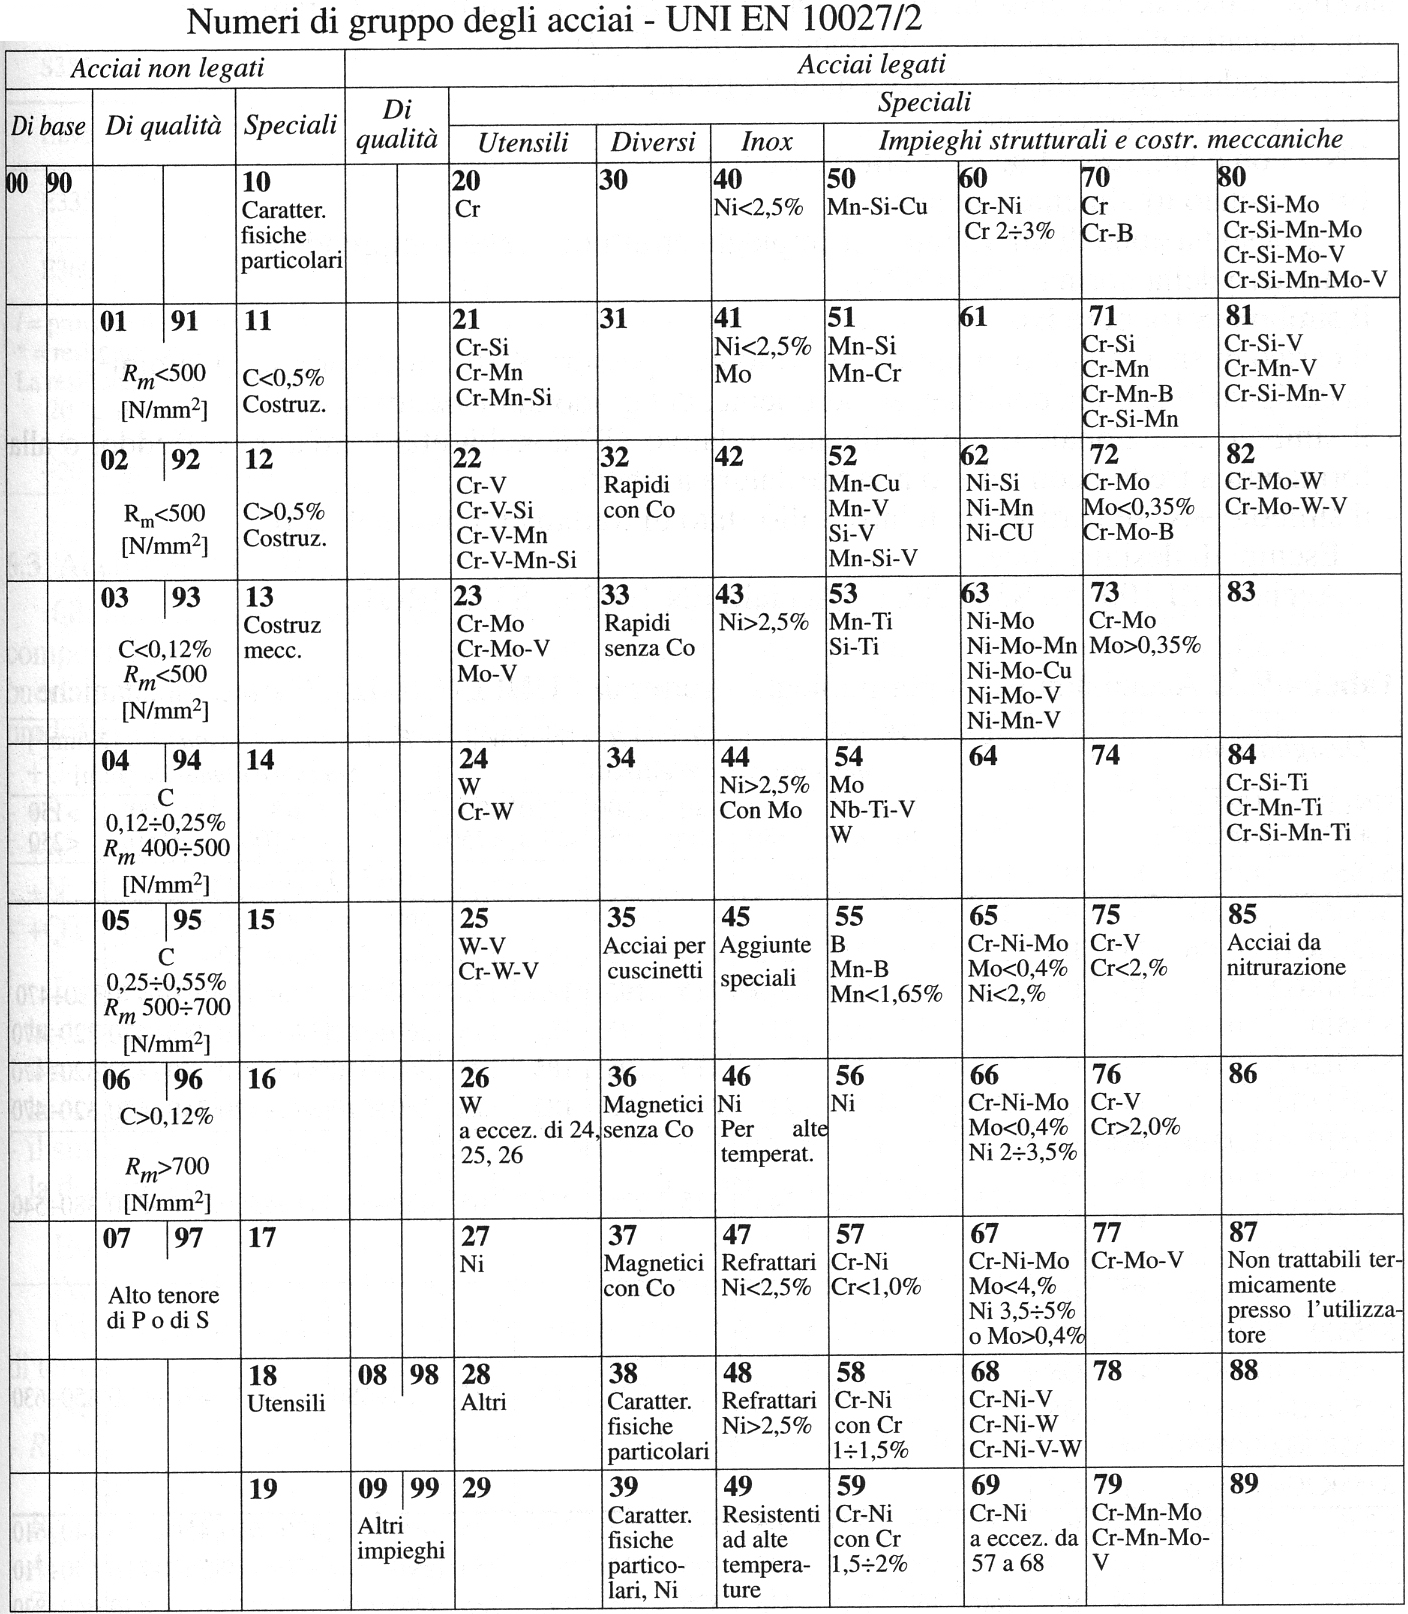
\includegraphics[width = \textwidth]{DesignazioneParte2}
\caption{Designazione acciai tramite UNI EN 10027-2}
\label{fig:UNIEN10027-2}
\end{figure}

\begin{example}{Esempi di designazione numerica}
\begin{description}
\item[1.0037] acciaio non legato equivalente al \texttt{S235JR}
\item[1.4306] acciaio inossidabile equivalente al \texttt{X2CrNi19-11}
\item[1.4401] acciaio inossidabile equivalente al \texttt{X4CrNiMo17-12-2}
\end{description}
\end{example}

Di seguito, alla figura \ref{fig:ConfDes}, viene riportato un confronto tra le varie modalità di designazione tra le normative.

\begin{figure}
\centering
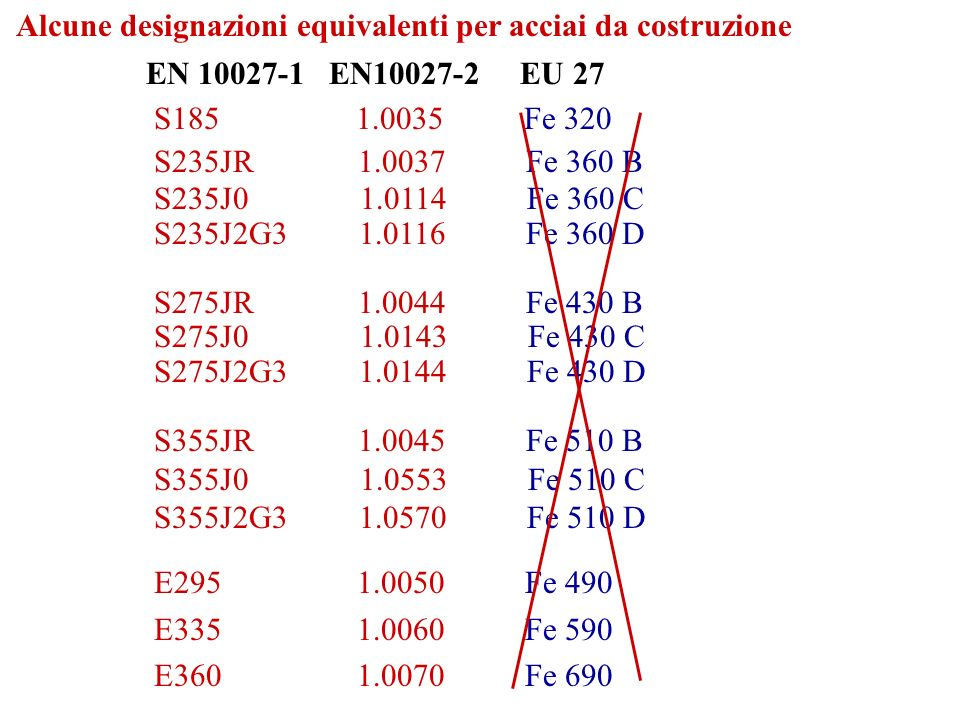
\includegraphics[width = \textwidth]{ConfrontoDesignazioni}
\caption{Confronto designazioni}\label{fig:ConfDes}
\end{figure}

\section{Cenni alla normativa AISI}\label{sc:AISI}
La designazione americana degli acciai deriva dal lavoro congiunto della \ac{AISI} e della \ac{SAE}.
Vediamo di seguuito il distinguo tra le varie categorie di acciai.

\subsection{Acciai al carbonio o basso legati}
Sistema numerico di 4 o 5 cifre: le prime due indicano la classe di appartenenza dell'acciaio. Le ultime due, o tre, indicano la $\%C \times 100$.

\begin{example}{Esempio designazione \ac{AISI}}
\begin{description}
\item[10XX(X)] acciai solo C
\item[41XX(X)] acciai al Cr-Mo
\end{description}
\end{example}

Può esserci una lettera di prefisso indicante il processo di fabbricaizone

\subsection{Acciai legati, ma sopratutto inox}
In questo caso si parla di una sigla a tre cifre con eventuale aggiunta delle lettere.
La prima cifra indica la classe, le altre due indicano una lega specifica.

\begin{example}{Esempi Norma AISI}
\begin{description}
\item[2XX] acciai austenitici Cr-Mn-Ni
\item[3XX] Inox austenitici Cr-Ni
\item[4XX] Inox martensitici o ferritici Cr
\end{description}
\end{example}

\section{Considerazioni generali}
la normativaa UNI EN 10027 non è sempre esaustiva: possono esserci dei casi in cui alcuni acciai non possano essere rappresentati tramite una solo stringa alfanumerica.
Si è osservato che diversi sono i punti di vista secondo i quali gli acciai possono essere classificati \emph{è evidente che non è possibile istituire una classificazione degli acciai che tenga conto di tutti questi aspetti}.

Ai fini pratici è indispensabile riferirsi alle applicazioni, pertanto si preferisce classificare gli acciai in 5 grandi categorie, suddivise a loro volta in classi.
\begin{itemize}
\item Acciai da costruzione di uso generale: acciai destinati a sopportare in opera sollecitazioni statiche o dinamiche senza rompersi o deformarsi oltre a limiti determinati.\\
In genere sono descritti dalla \ref{ssc:10027-1Gruppo1}.
\item Acciai speciali da costruzione: acciai destinati ad applicazioni più impegnative, nelle quali esplicano sopratutto la funzione di resistere a carichi statici e dinamici. In generale appartengono alle sottocategorie \ref{sssc:Sottogruppo2.1} e \ref{sssc:Sottogruppo2.2} alcuni particolari casi anche alla \ref{sssc:Sottogruppo2.3} perché nessun elemento in lega supera la soglia del $5\%$ di tenore.
\item Acciai inossidabili: acciai destinati a resistere a determinate condizioni lavorative in ambienti corrosivi. Appartengono alla \ref{sssc:Sottogruppo2.3}.
\item Acciai da utensili destinati alle lavorazioni di tutte le classi di materiali. Appartengono a diverse classi a seconda di quale sia la loro applicazione, dunque si trovano in: \ref{sssc:Sottogruppo2.2}, \ref{sssc:Sottogruppo2.3} e \ref{sssc:Sottogruppo2.4}
\item Acciai per usi particolari: acciai caratterizzati dal fatto che il loro impiego è determinato da alcune loro singolari proprietà. Ad esempio: acciai per impieghi a basse temperature, acciai refrattari, acciai con particolari proprietà elettriche o magnetiche ecc\dots
\end{itemize}